\section{Selectivity and Optimization Principle}
\subsection{Question (Paper \& Pencil)} 

We can write the gradient descent on the objective function F($\omega$) as:
\begin{eqnarray}
\Delta \omega&=&\eta \frac{\partial F(\omega)}{\partial \omega} \\
&\approx&\frac{\partial }{\partial \omega} \left\langle \left(\frac{y}{\sigma_y}\right)^3 \right\rangle \\
&\approx&\frac{\partial }{\partial \omega} \left\langle \left(\frac{y}{\sqrt{\langle y^2\rangle}}\right)^3 \right\rangle \\
&\approx&\frac{\partial }{\partial \omega} \left\langle \frac{y^3}{\langle y^2\rangle  \sqrt{\langle y^2\rangle}} \right\rangle
\end{eqnarray}

using the given $\sigma_y = \sqrt{\langle y^2\rangle}$. Using the distributive properties of the expectation operation (i.e. $\langle A + B \langle C\rangle\rangle = \langle A  \rangle + \langle B\rangle \langle C\rangle$ and $\left\langle \frac{A}{\langle B\rangle}\right\rangle = \frac{\langle A  \rangle}{\langle B  \rangle}$ we can write Eq. \ref{eq:distri}: 

\begin{eqnarray}
\Delta \omega&\approx& \frac{\partial }{\partial \omega}  \frac{\langle y^3 \rangle}{\langle y^2 \rangle \langle \sqrt{\langle y^2 \rangle}\rangle}  \label{eq:distri}\\
\end{eqnarray}

and knowing $\theta = \frac{\langle y^3\rangle}{\langle y^2\rangle}$, 
\begin{eqnarray}
\Delta \omega&\approx& \frac{\partial }{\partial \omega}  \frac{\theta}{ \langle \sqrt{\langle y^2 \rangle}\rangle} \\
\end{eqnarray}

taking the derivative yields: 
\begin{eqnarray}
\Delta \omega&\approx& \frac{\partial \theta}{\partial \omega}  \frac{1}{ \langle \sqrt{\langle y^2 \rangle}\rangle} -  \frac{\theta}{2}  {\langle y^2 \rangle}^{-3/2} \langle 2y x \rangle \label{eq:delta_omega}
\end{eqnarray}

now noticing $\langle {\langle y^2 \rangle}^{1/2} \rangle$ has an outer expectation value operation on a scalar, we can write $ {\langle y^2 \rangle}^{1/2} $ instead.

Partial derivative of $\theta$ with respect to $\omega$:

\begin{eqnarray}
\frac{\partial \theta}{\partial \omega} &=& \frac{\langle 3y^2 x\rangle}{\langle y^2 \rangle}  - \frac{\langle y^3\rangle}{\langle y^2\rangle^2} \langle 2yx\rangle \\
 &=& \frac{3\langle y^2 x\rangle}{\langle y^2 \rangle}  - \frac{\theta}{\langle y^2\rangle} 2\langle yx\rangle \\
 &=& \frac{3\langle y^2 x\rangle-2\theta\langle yx\rangle}{\langle y^2 \rangle}  \label{eq:partial_theta}
\end{eqnarray}

If we use Eq. \ref{eq:partial_theta} in Eq. \ref{eq:delta_omega}, we get: 
\begin{eqnarray}
\Delta \omega&\approx&  \frac{3\langle y^2 x\rangle-2\theta\langle yx\rangle}{\langle y^2 \rangle^{3/2}}   -  \frac{\theta \langle y x \rangle}  {\langle y^2 \rangle^{3/2}} \\
\Delta \omega&\approx&  3\frac{\langle y^2 x\rangle-\theta\langle yx\rangle}{\langle y^2 \rangle^{3/2}}  \label{eq:final_form} 
\end{eqnarray}

where Eq. \ref{eq:final_form} is of the form $\dot\omega =  xy^2 - xy\theta$.
\newpage
\subsection{Question (Simulation)}

\begin{figure}[h]
\centering
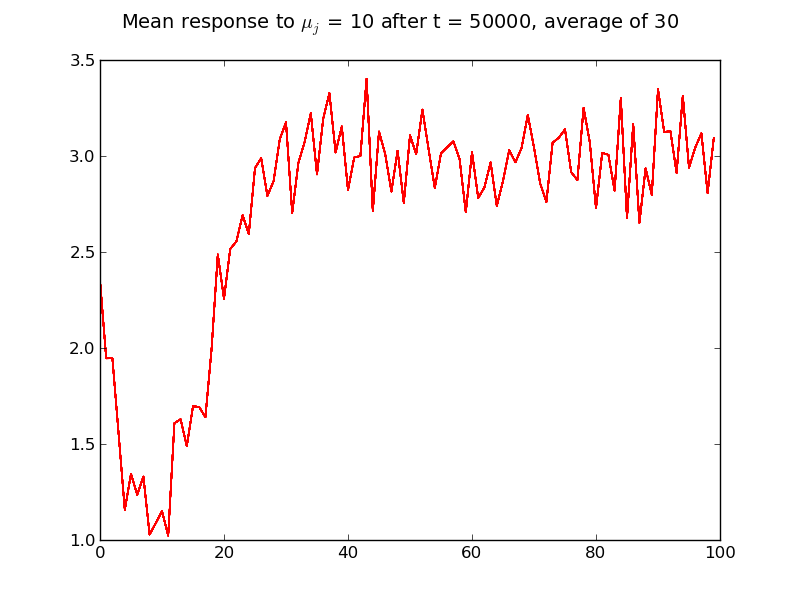
\includegraphics[width=0.7\textwidth]{../ex2/weights_mu10_t50k_mean.png}
\caption{TEXT HERE}
\label{fig:mu10}
\end{figure}

\begin{figure}[h]
\centering
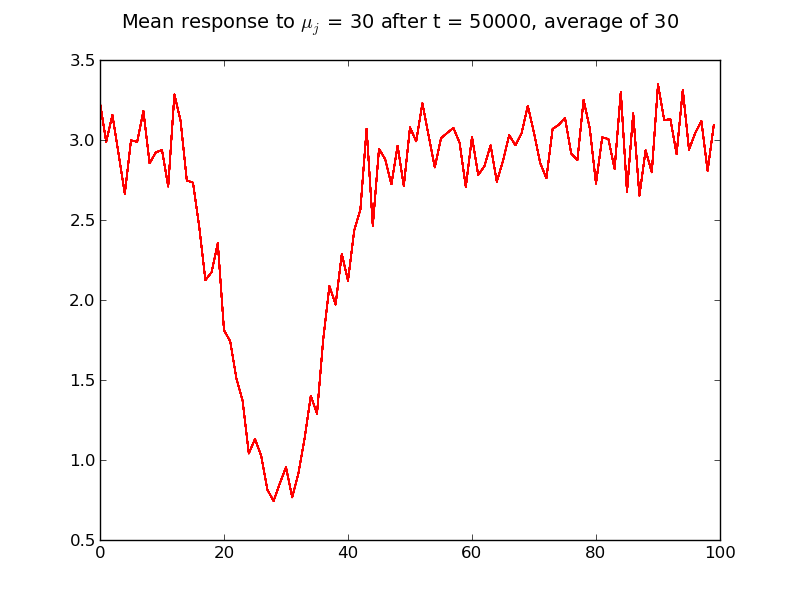
\includegraphics[width=0.7\textwidth]{../ex2/weights_mu30_t50k_mean.png}
\caption{TEXT HERE}
\label{fig:mu30}
\end{figure}

\begin{figure}[h]
\centering
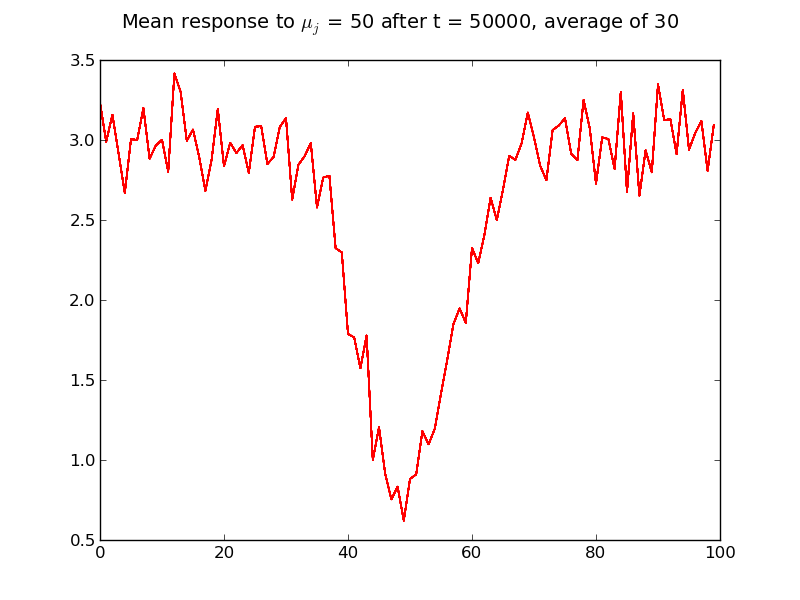
\includegraphics[width=0.7\textwidth]{../ex2/weights_mu50_t50k_mean.png}
\caption{TEXT HERE}
\label{fig:mu50}
\end{figure}

\begin{figure}[h]
\centering
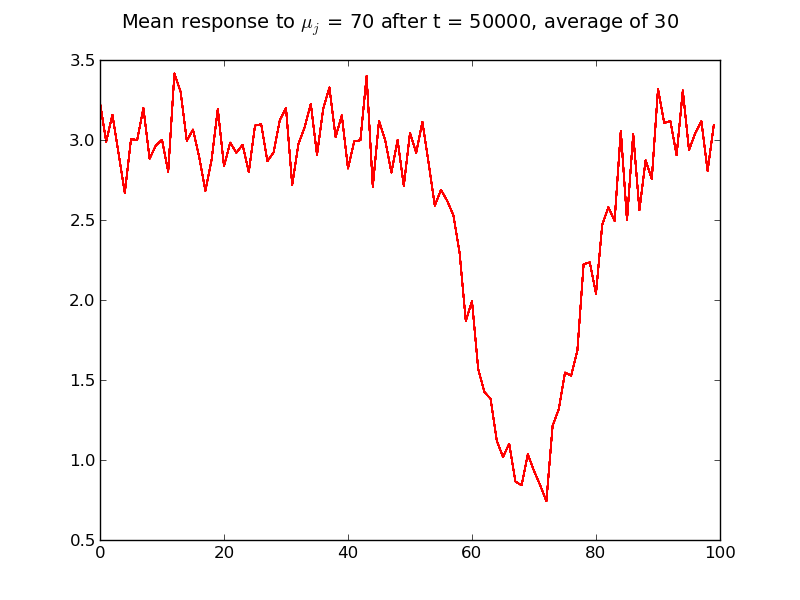
\includegraphics[width=0.7\textwidth]{../ex2/weights_mu70_t50k_mean.png}
\caption{TEXT HERE}
\label{fig:mu70}
\end{figure}

\begin{figure}[h]
\centering
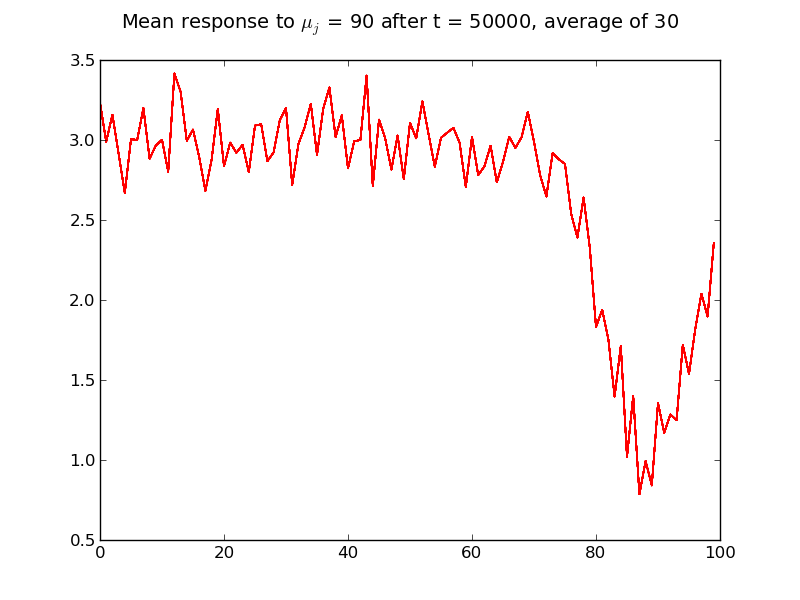
\includegraphics[width=0.7\textwidth]{../ex2/weights_mu90_t50k_mean.png}
\caption{TEXT HERE}
\label{fig:mu90}
\end{figure}
